%grundlagen.tex

\chapter{Grundlagen}
\label{chapter:gru}

\section{Chromatographie}

Die Chromatographie ist ein Verfahren zur Auftrennung von Stoffgemischen. 
Die Auftrennung erfolgt dabei zwischen zwei sogenannten Phasen, der stationären und der mobilen Phase, welche sich in unterschiedlichen Aggregatzuständen befinden und untereinander nicht mischen. 

Es existieren zum einen die Flüssigchromatographie (LC, engl. Liquid Chromatography),
\todo{Muss englische Worterklärung kursiv oä?}
bei der die mobile Phase eine Flüssigkeit ist und die stationäre Phase ein Feststoff. Bei der Gaschromatographie (GC) ist die mobile Phase ein Gas und es wird zusätzlich nach der stationären Phase unterschieden. Ist diese ein Feststoff, so spricht man von gepackten Säulen. Bei der Kapillartechnik hingegen werden die Trennsäulen innen mit einem Flüssigkeitsfilm als stationäre Phase beschichtet.




% Die Gaschromatographie (GC) ist ein Verfahren, mit dem gasförmig vorliegende Stoffgemische aufgetrennt oder analysiert werden können. 
% Die Auftrennung erfolgt dabei zwischen zwei sogenannten Phasen, der stationären und der mobilen Phase, welche sich in unterschiedlichen Aggregatzuständen befinden und untereinander nicht mischen. 



% Allgeinprinzip: Phasen, Phasenwechsel
% Arten der Chroma -> Interessant GC mit Kapillartechnik
% Detektion / Weiterverarbeitung
% Probleme: Peakshapes (Tailing), Ursache
% Verwandte Arbeiten?
% Wo kommt das mit den Referenzdatensätzen rein?

Beispielsweise kann die GC in einer Multikapillarsäule (MCC, engl. Multi Capillary Colum) stattfinden. Sie besteht aus ca. 1000 \todo{Quelle Anzahl Kapillaren einer MCC} einzelnen Kapillaren. Jede davon ist innen mit der sog. stationären Phase beschichtet. Außerdem kommt ein Trägergas, die sog. mobile Phase, zum Einsatz, welches die Analyte durch die Säule transportiert. 

\subsection{Der chromatograpische Prozess}
Die Substanzen unterscheiden sich vor allem durch ihre Wechselwirkungen mit der stationären Phase. Während dieser Wechselwirkungen haften die Teilchen an der stationären Phase, bewegen sich also nicht fort. Finden wenig Wechselwirkungen statt, passieren die Teilchen die Säule schneller, als wenn viele Wechselwirkungen stattfinden. Dies beeinflusst die Retentionszeit, also die Zeit, die zum Durchlaufen der Säule gebraucht wird.
\todo{Ausführlich den chroma Proz beschreiben}

%\todo{Wegen Datensätzen muss das doch rein
\subsection{Detektion}
Nach Durchlaufen der Säule wird detektiert, welche Menge an Substanzen austreten. Dabei wird nicht die Art des Analyts festgestellt, sondern nur die Menge der zum jeweiligen Zeitpunkt austretenden Stoffe. Dabei zeichnet der Detektor ein Chromatogramm auf, welches beispielhaft in \todo{Bild Chromatogramm} zu sehen ist

Alternativ kann die Gaschromatographie auch als Vorverarbeitung für Verfahren wie Massenspektrometrie (MS) oder Ionen-Mobilitäts-Spektrometrie (IMS) dienen. In diesen Fällen werden die aus der MCC austretenden Moleküle direkt ionisiert und in den entsprechenden Geräten weiter analysiert.

Die für diese Arbeit vorliegenden Referenzdatensätze stammen aus einer solchen MCC-IMS-Kopplung. Ein Beispiel dafür ist in \ref{picture:Spektrum1} zu sehen. \todo{Spektrum erklären}
\begin{figure}
 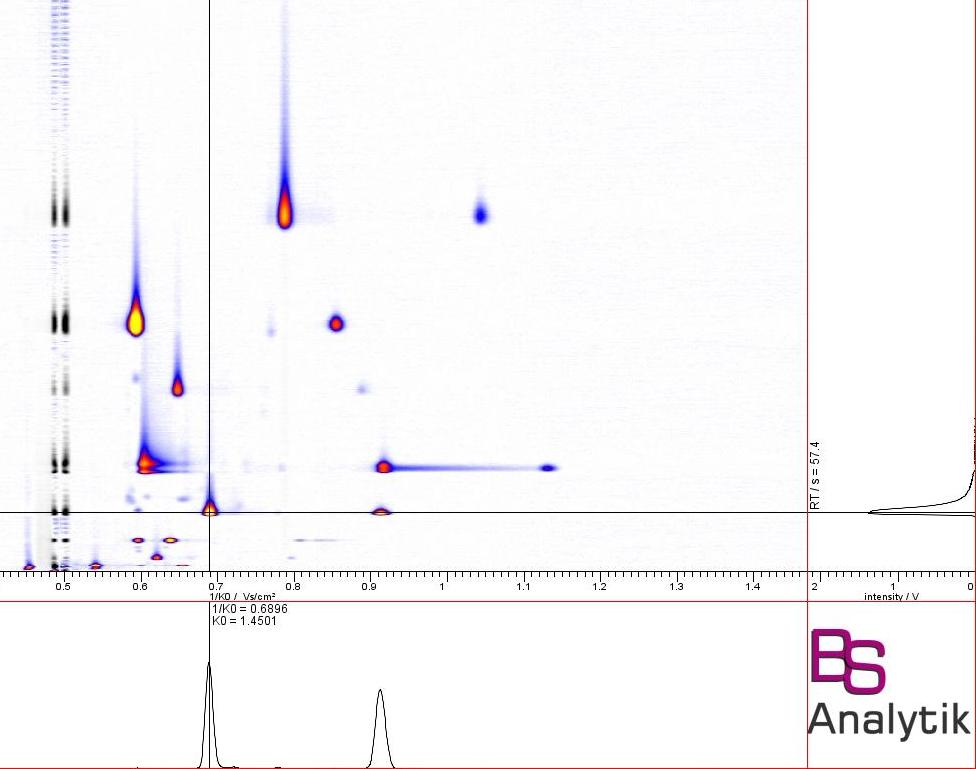
\includegraphics[width = 0.9\textwidth]{bilder/BD15_1304101102_ims}
 \caption{Spektrum einer MCC-IMS-Messung}
 \label{picture:Spektrum1}
\end{figure}
%
Zu beobachten ist, dass schnelle Teilchen Peaks zu frühen Zeitpunkten erzeugen, die eine relativ geringe Varianz aufweisen, hingegen spätere Peaks tendenziell breiter werden. Ideale Peaks haben die Form einer Gaußkurve.


\subsection{Peakcharakteristika}
Um später die simulierten Peaks mit denen aus den Referenzdatensätzen gut vergleichen zu können, sollen nun einige Eigenschaften aufgeführt werden, die einen Peak beschreiben.

Die offentsichtlichste Eigenschaft ist die Lage des Peaks, genauer gesagt, die Lage des Maximums des Peaks.

Außerdem können die Peaks verschiedene Formen haben. Im theoretischen Idealfall haben sie die Form einer Gaußkurve, jedoch tritt oft ein Tailing auf, welches verschiedene Ursachen haben kann. Unter Anderen seien hier genannt: zusätzliche Adsorptionseffekte, die beim Altern einer Säule auftreten \cite{kolb2003}, technische Ursachen wie kleinste Hohlräume zwischen der Säule und dem Gaseinlass bzw. -Austritt, sowie einige Stoffe, die generell zu Tailing neigen \todo{Zitat, dass einige Stoffe gererell tailen}. 
Beim Tailing steigt die Kurve zunächst stark an, sinkt jedoch nach Erreichen des Maximalwerts deutlich langsamer ab, es entsteht ein Schwanz (engl. Tail). Auch der umgekehrte Fall, Fronting genannt, kann auftreten, ist jedoch in den vorliegenden Datensätzen nicht zu beobachten.

Als drittes können Peaks unterschiedlich breit sein. Da jedoch ein Peak mit größerer Intensität, also möglicherweise größerer Stoffmenge, automatisch auch einen breiteren Peak erzeugt, betrachten wir die Halbwertsbreite als Maß für die Peakbreite. Die Halbwertsbreite wird auf halber Maximalhöhe des Peaks gemessen. Im Fall von auftretendem Tailing oder Fronting ist es sinnvoll, je einen Wert für rechts und links des Maximalwerts zu berechnen.


\section{Probabilistische Arithmetische Automaten}
Ein Probabilistischer Arithmetischer Automat (PAA) nach \cite{MHKR} ist ein Modell, mit dem eine Folge zufälliger Operationen beschrieben werden kann. 
Für PAA existieren Algorithmen, welche eine gemeinsame Verteilung von Zuständen und Werten oder auch die Verteilung der Wartezeit für einen Wert berechnen. Wie in Kapitel \ref{chapter:mod} beschrieben wird, kann das Modell zur Simulation einer Multikapillarsäule auch als PAA formuliert werden. Mit dieser Formulierung ist die Zeit, die zum Durchlaufen einer Säule gebraucht wird, dann die Wartezeit für den Wert, welcher der Länge der Säule entspricht. Deshalb kann ein PAA nützlich sein, um neben der eigentlichen Simulation auch noch eine erwartete Verteilung der Ankunftszeiten der Teilchen zu berechnen. 

Zunächst sei hier eine Definition für den PAA gegeben, anschließend wird der Algorithmus zur Berechnung der Wartezeit beschrieben.
%In diesem Fall ist die Länge der Säule der Wert, auf den gewartet wird und man ist interessiert in der Verteilung der Anzahl der Zeitschritte, die benötigt werden, um die Länge zu erreichen. 

%TODO: Wo soll das rein? Sinnvoll, wenn das zu Beginn erklärt
% Was tut ein PAA

\subsection{Definition eines PAA}
% Formale Definition

\begin{definition}[PAA]
 Ein Probabilistischer Arithmetischer Automat (PAA) ist ein Tupel
 $ \mathcal{P} = (\mathcal{Q}, q_0, T, \mathcal{V}, v_0, \mathcal{E}, (e_q)_{q\in\mathcal{Q}}, (\theta_q)_{q\in\mathcal{Q}})$, dabei ist:
 \begin{itemize}
  \item $\mathcal{Q}$ eine endliche Menge von Zuständen
  \item $q_0 \in \mathcal{Q}$ der Startzustand
  \item $T: \mathcal{Q} \times \mathcal{Q} \rightarrow [0,1]$ eine Übergangsfunktion mit $\sum_{q' \in \mathcal{Q}} T(q, q') = 1 $ das heißt $(T(q,q'))_{q,q' \in \mathcal{Q}}$ ist eine stochastische Matrix
  \item $\mathcal{E}$ eine endliche Menge von Emissionen
  \item $e_q: \mathcal{E} \rightarrow [0,1]$ eine Wahrscheinlichkeitsverteilung der Emissionen für jeden Zustand
  \item $\mathcal{V}$ eine Menge von Werten
  \item $v_0$ der Startwert
  \item $\theta_q: \mathcal{V} \times \mathcal{E} \rightarrow \mathcal{V}$ eine Operation für jeden Zustand
 \end{itemize}
\end{definition}
Dabei entspricht $ \mathcal{P} = (\mathcal{Q}, q_0, T)$ einer Markovkette und $ \mathcal{P} = (\mathcal{Q}, q_0, T, \mathcal{E}, (e_q)_{q\in\mathcal{Q}})$ einem Hidden Markov Model. \todo{Muss ich dann Markov erklären?}

\subsection{Algorithmus zur Berechnung der Wartezeit}

\todo{Algos für die Verteilung und Wartezeit-Berechnung vorstellen}